\section{Clustering}
\label{sec:clustering}

In order to identify patterns in the trip data, we clustered trips using kmeans++ and gaussian mixture models. This can help in identifying local hotspots or recurring trips types such as commutes or leisure trips. 

Kmeans++ is a hard clustering algorithm that assigns each data point to a definite cluster. Gaussian mixture models (GMMs), on the other  hand, are a soft clustering algorithm meaning we compute the probabilities of each data point belonging to each clusters. This gives us a measure of uncertainty. Moreover, while kmeans is mostly suited for capturing spherical shapes, GMM are also able to detect ellipsis shapes. However, non-convex shapes pose a difficulty for both algorithms. GMMs also tend to have longer computation times than kmeans due to the increased complexity. 
In this section, we discuss the results of the hard clustering and soft clustering analysis. We clustered the data using all features in the first step and based on feature subsets in the second step. However, in this paper we only present the clustering using all features. We also omit plotting weather data, minimum distance and minimum average speed, which was also used in the clustering, as it did not yield any interesting insights. 

\subsection{Hard Clustering}
\label{sec:hard_clustering}


\begin{figure}[htp]
    \centering
    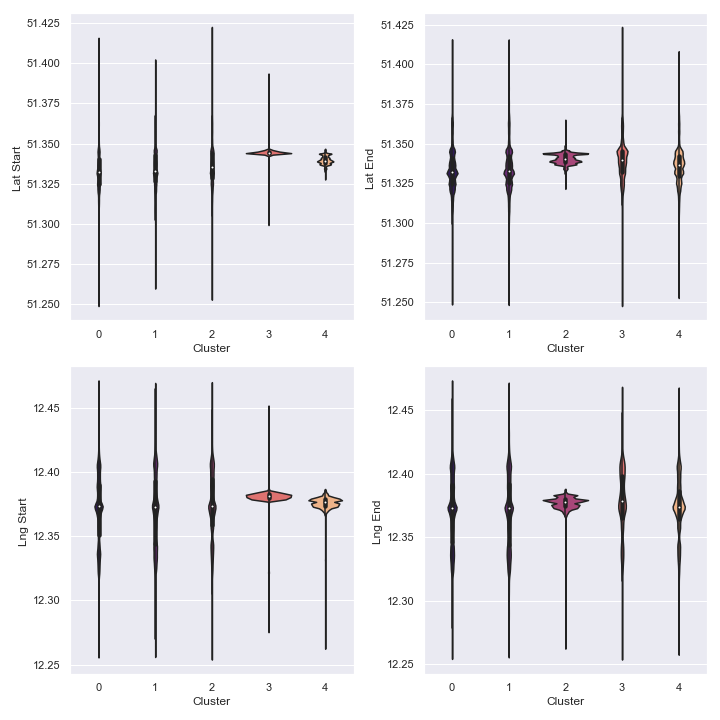
\includegraphics[width=0.48\textwidth]{Figures/Clustering/clusters_lat_start.png}
    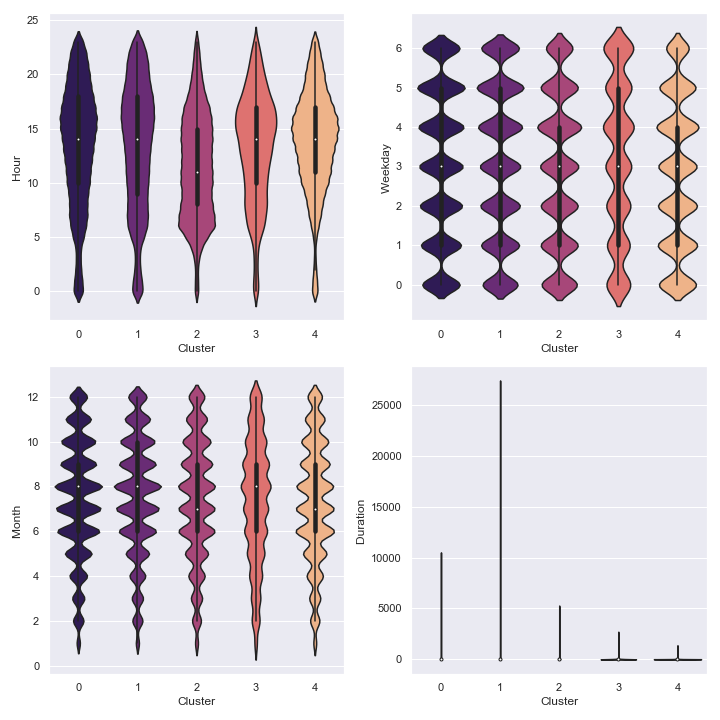
\includegraphics[width=0.48\textwidth]{Figures/Clustering/clusters_hour.png}
    \caption{Kmeans Clustering - Location And Temporal Features}
    \label{fig:kmeans_loc_temp}
\end{figure}

-cluster 0: 
-cluster 1: long trips (not on average but outliers), 
-cluster 2: start a city center, early, during the week, short 
-cluster 3:go to city center
-cluster 4:go to city center, during the week

\begin{figure}[htp]
    \centering
    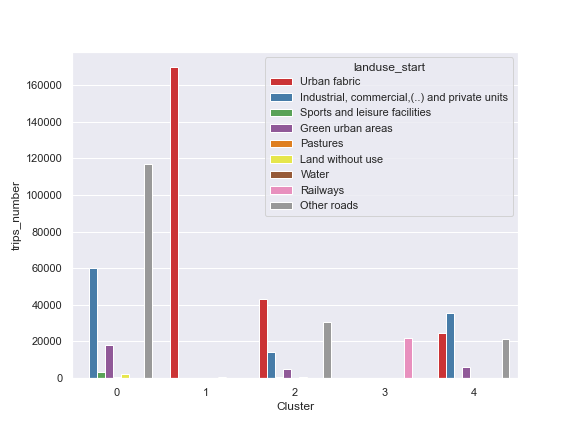
\includegraphics[width=0.48\textwidth]{Figures/Clustering/landuse_start.png}
    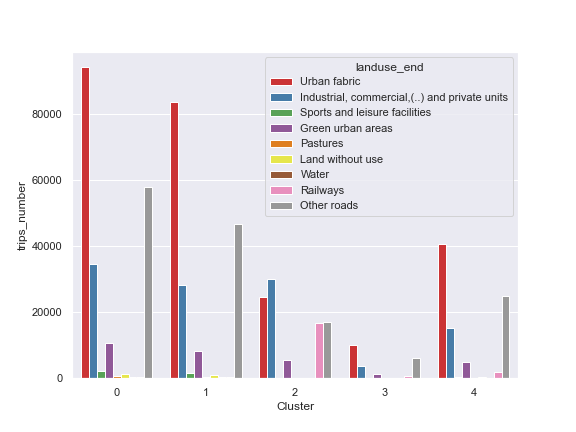
\includegraphics[width=0.48\textwidth]{Figures/Clustering/landuse_end.png}
    \caption{Kmeans Clustering - Land Use Start and End}
    \label{fig:kmeans_land_use}
\end{figure}

-cluster 0: largest cluster, start from roads and go to urban fabric 
-cluster 1: start in urban fabric,
-cluster 2: got to railway or urban/ industrial areas, 
-cluster 3:start at railway
-cluster 4:

\begin{figure}[htp]
    \centering
    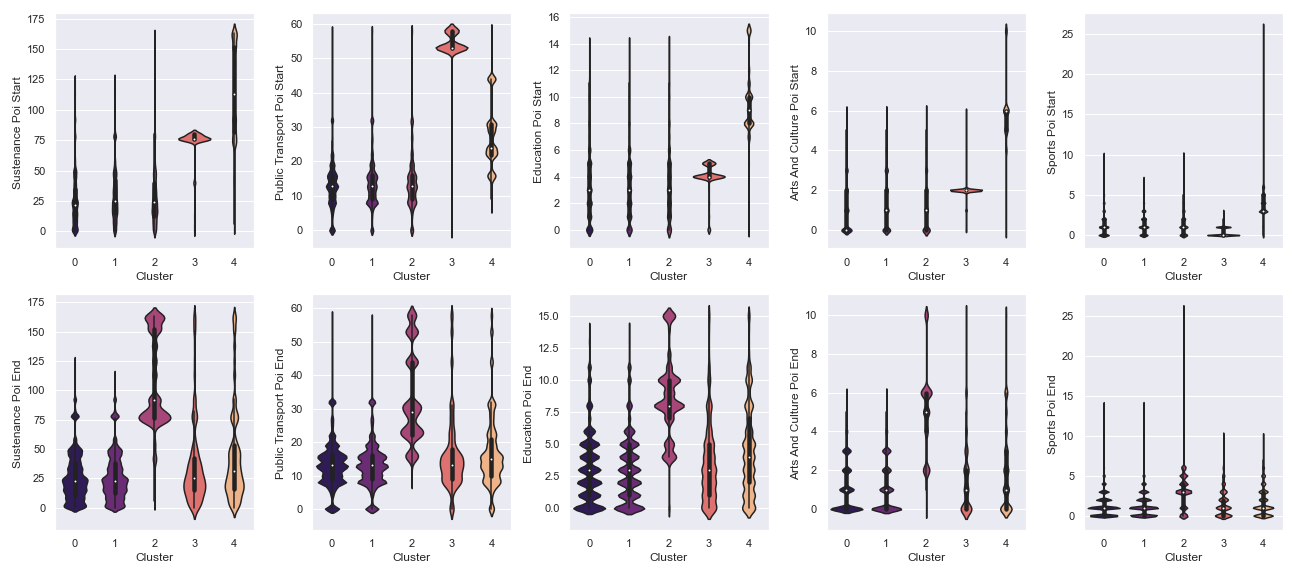
\includegraphics[width=0.9\textwidth]{Figures/Clustering/clusters_sustenance_poi_start.png}
    \caption{Kmeans Clustering - Points Of Interest}
    \label{fig:kmeans_poi}
\end{figure}

-cluster 0: 
-cluster 1: 
-cluster 2: to a lot of pois (working areas)
-cluster 3: start at public transport (railway)
-cluster 4: starts at sustenance poi, (also arts/culture, sports, education), 